\documentclass{article}
\usepackage{url}
\usepackage{amsmath,bm}%
\usepackage{amsfonts}%
\pagestyle{empty}
\setlength{\textwidth}{7in}
\setlength{\oddsidemargin}{-.5in}
\setlength{\evensidemargin}{-.5in}
\setlength{\topmargin}{-.75in}
\setlength{\textheight}{9.25in}

\newcommand{\beaa}{\begin{eqnarray*}}
\newcommand{\eeaa}{\end{eqnarray*}}
\newcommand{\bea}{\begin{eqnarray}}
\newcommand{\eea}{\end{eqnarray}}
\def\E{\mathop{\rm E\,}\nolimits}
\def\Var{\mathop{\rm Var\,}\nolimits}
\def\Cov{\mathop{\rm Cov\,}\nolimits}
\def\Corr{\mathop{\rm Corr\,}\nolimits}
\def\logit{\mathop{\rm logit\,}\nolimits}
\newcommand{\eid}{{\stackrel{\cal{D}}{=}}}
\newcommand{\cip}{{\stackrel{{P}}{\to}}}
\def\bR{\mathbb{R}}     % real line

\usepackage{Sweave}
\begin{document}

\begin{center}
{\bf STAT 515}

{\bf Homework \#6 WITH SOLUTIONS}

\end{center}

\begin{enumerate}

\item Let $N(t)$ be a non-homogeneous Poisson process with rate function
$\lambda(t)$.

  \begin{enumerate}

  \item Fix some $t>0$. Derive the conditional distribution of the arrival times
  $S_1, \ldots, S_{N(t)}$, conditional on $N(t)=n$.
  \begin{quotation}{\bf Solution:} 
  There are a couple ways to obtain this.  One is to employ the 
  argument used in the textbook for the case of the homogeneous Poisson process.
  For $0<s_1< \cdots < s_n < t$,
  the event $S_1=s_1, \ldots, S_n=s_n$ is the same as the event  
  \[
  T_1=s_1, T_2 = s_2-s_1, \ldots, T_n=s_n-s_{n-1}, T_{n+1}>t-s_n.
  \]
  Therefore, by the independence of the $T_i$, we can find the density function
  by multiplying the densities:
  \[
  f_{S_1, \ldots, S_{N(t)} \mid N(t)=n}(s_1, \ldots, s_n) = 
  \frac{1}{P(N(t) = n)}
  \prod_{i=1}^n f_{T_i \mid S_{i=1}=s_{i-1}} (s_i-s_{i-1}) P(T_{n+1}>t-s_n \mid S_n=s_n).
  \]
  Thus, it is necessary to find the conditional density of $T_i$ conditional on $S_{i=1}-s_{i-1}$.
  From the non-homogeneous Poisson process theory, we know that the conditional cdf
  is 
  \[
  F_{T_i \mid S_{i=1}=s_{i-1}} (a)
  = 1 - P\{\mbox{No events in $(s_{i-1}, a]$} \} 
  = 1-\exp\{m(s_{i-1})-m(a)\} \quad \mbox{for $a>s_{i-1}$,}
  \]
  where $m(a) = \int_0^a \lambda(u)\,du$.  This gives (since $m'(a)=\lambda(a)$)
  \[
  f_{T_i \mid S_{i=1}=s_{i-1}} (a) = [\lambda(a)]\exp\{m(s_{i-1})-m(a)\} \quad \mbox{for $a>s_{i-1}$}
  \]
  as the conditional density function.  Substituting into the expression above gives
  \[
  f_{S_1, \ldots, S_{N(t)} \mid N(t)=n}(s_1, \ldots, s_n) = 
  \frac{n!}{\exp\{-m(t)\} [m(t)]^n}
  \prod_{i=1}^n \biggl( [\lambda(s_i)]\exp\{m(s_{i})-m(s_{i-1})\}  \biggr)
  \exp\{ m(s_n) - m(t) \}.
  \]
  A lot of cancellation happens in the above product, and we are left with
    \[
  f_{S_1, \ldots, S_{N(t)} \mid N(t)=n}(s_1, \ldots, s_n) = n!
  \prod_{i=1}^n \left[ \frac{\lambda(s_i)}{m(t)} \right].
  \]
  This is the joint density of the order statistics of an i.i.d.~sample of random variables
  $X_1, \ldots, X_n$ with density function $f(x) = \lambda(x)/m(t)$ for $0<x<t$.
  \end{quotation}

  \item As you did in Exercise 2(a) of Homework \#5, use part (a) to suggest an
  algorithm for simulating a non-homogeneous Poisson process on $(0, t]$.
  \begin{quotation}{\bf Solution:}
  Step one:  Simulate $N(t)$, which is Poisson$\{m(t)\}$.  Step two:  Generate an 
  i.i.d.~sample of size $N(t)$ from the density $f(x)=\lambda(x)/m(t)$.  These sample points
  are then the times of the events in the non-homogeneous Poisson process.
  \end{quotation}

  \item Use your algorithm to simulate 10,000 realizations of a non-homogeneous
  Poisson process on $(0, 2]$ where $\lambda(t) = 24t^2$.
  \begin{quotation}{\bf Solution:}
  Since $\lambda(x)/m(t)$ is proportional to $x^2$ and $0<x<2$, the density of the
  i.i.d.~sample will be that of two times a beta$(3,1)$ random variable.  Also, the mean 
  number of events in $(0,2]$ is $m(2)$, which equals 
  $24 \int_0^2 u^2\,du = 8(2^3) = 64$.  Therefore, we obtain:
\begin{Schunk}
\begin{Sinput}
> X <- list()  # Use double-brackets to refer to list items, e.g., X[[1]]
> for (i in 1:10000) {
+   X[[i]] <- sort(2*rbeta(rpois(1, 64), 3, 1))
+ }
\end{Sinput}
\end{Schunk}
  \end{quotation}

  \item Using the result of part (c), produce a histogram of the numbers of
  events in the interval $(0, 1]$. Add to your histogram the true theoretical
  values, and explain how you found them.
  \begin{quotation}{\bf Solution:}
  
\begin{Schunk}
\begin{Sinput}
> f0 <- function(vec) sum(0<vec & 1>vec)
> ans0 <- sapply(X, f0)
> mean(ans0) + c(-1, 1) * 1.96 * sd(ans0)/ sqrt(length(ans0))
\end{Sinput}
\begin{Soutput}
[1] 7.9181 8.0273
\end{Soutput}
\begin{Sinput}
> hist(ans0, breaks=0.5+(min(ans0)-1):max(ans0), main="Events in (0,1]", xlab="")
> x0 <- min(ans0):max(ans0)
> lines(x0, 10000*dpois(x0, 8), col=2, type="b")
\end{Sinput}
\end{Schunk}
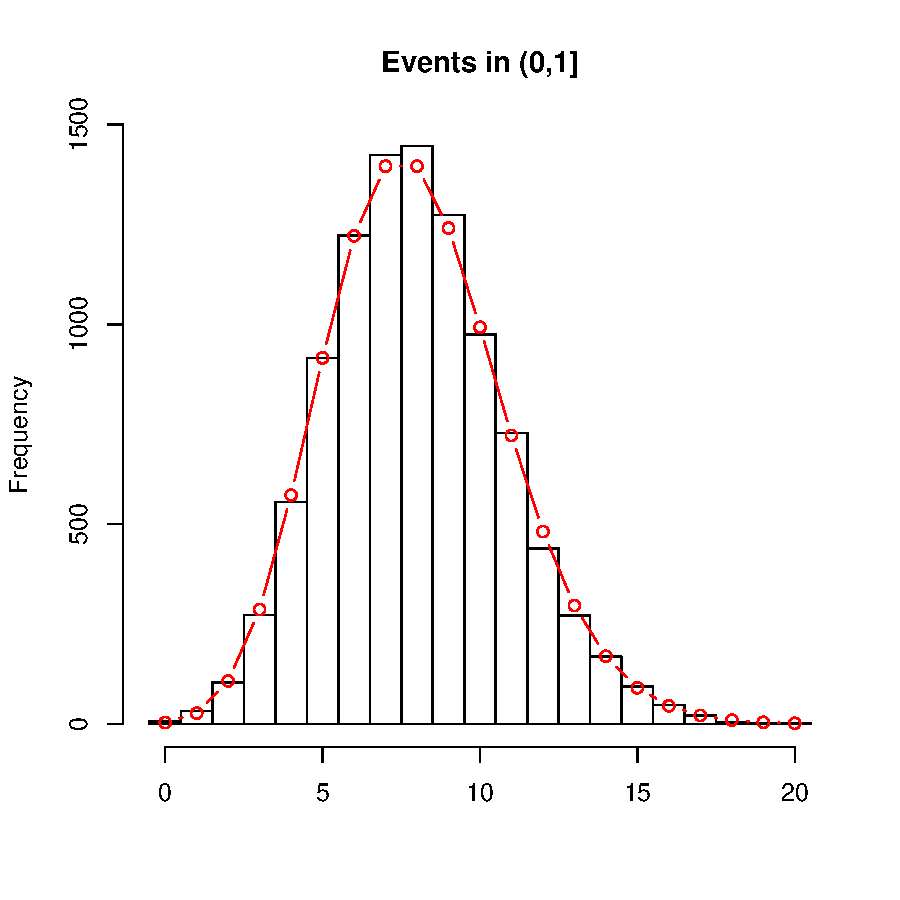
\includegraphics{sol06-002}
  \end{quotation}

  \item Using the result of part (c), produce a histogram of the times until the
  first event. Add to your histogram the true theoretical density, and explain
  how you found it. What is the name of the true theoretical distribution?
  \begin{quotation}{\bf Solution:}
  From the argument in part (a), we know that the cdf of $T_1$ is
  $F(x) = 1- \exp\{-m(x)\}$.  In this case, with $m(x)=8x^3$,
  the cdf is recognizable as a Weibull distribution with shape parameter
  $3$ and scale parameter $1/2$.
  In the plot below, the red curve is the true Weibull density and the green curve
  is an estimated density curve based on the data only.
\begin{Schunk}
\begin{Sinput}
> ans1 <- sapply(X, min)
> hist(ans1, main="Time until first event", xlab="", freq=FALSE)
> s <- seq(min(ans1), max(ans1), len=200)
> lines(density(ans1), col=3, lwd=2) # Add a kernel density estimate (green)
> lines(s, dweibull(s, 3, 0.5), col=2, lwd=2) # True Weibull density (red)
\end{Sinput}
\end{Schunk}
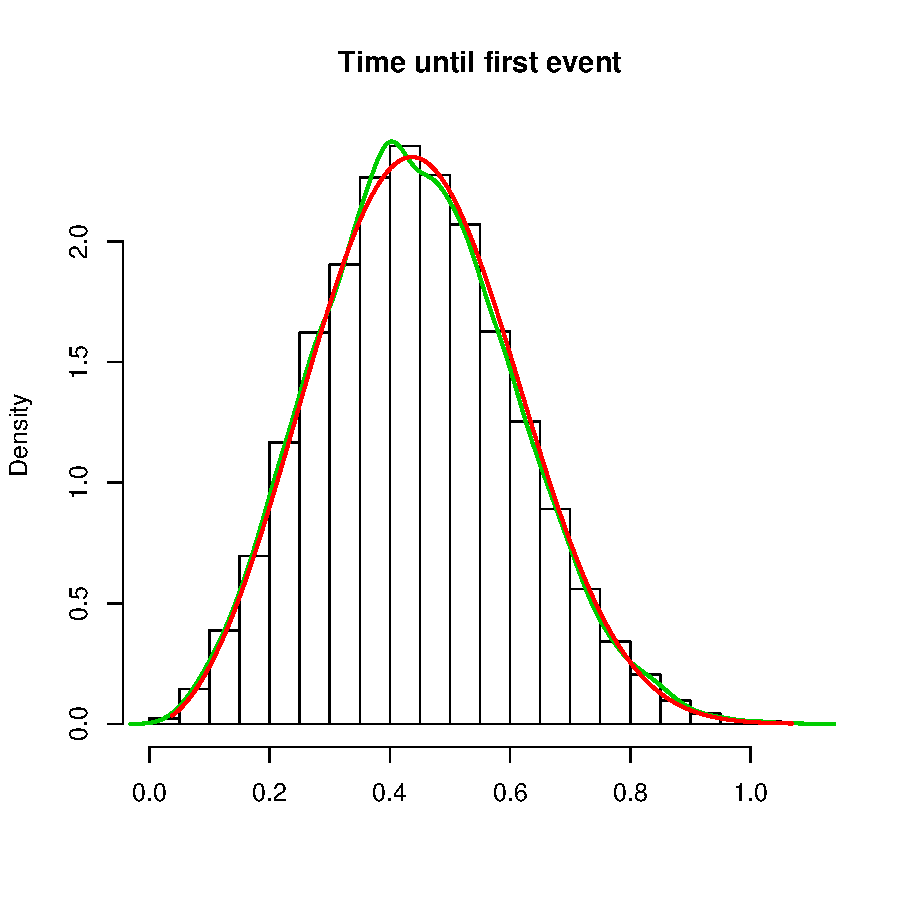
\includegraphics{sol06-003}
  \end{quotation}

  \end{enumerate}  

\item Teams 1 and 2 are playing a game. The teams score points according to
independent Poisson processes with rates $\lambda_1$ and $\lambda_2$,
respectively. The game ends when one team has scored exactly $k$ points more
than the other team. What is the probability that team 1 wins?
  \begin{quotation}{\bf Solution:}
  In this case, the Poisson process theory states that at any given instant, the probability
  that team 1 scores the next point equals $\lambda_1/(\lambda_1+\lambda_2)$,
  independently of the entire past.  This means that we have a gambler's ruin problem:
  It is as though team 1 starts with $k$ points, wins a point at each step with probability
  $\lambda_1/(\lambda_1+\lambda_2)$ and loses a point with the complementary probability, 
  and wins the entire game if it gets to
  $2k$ points before it gets to 0 points.  Using results from the textbook, we conclude that
  \[
  P(\mbox{team 1 wins the game}) = 
  \begin{cases}
  \frac{1 - (\lambda_2/\lambda_1)^k}{1 - (\lambda_2/\lambda_1)^{2k}} & 
  \mbox{if $\lambda_1\ne\lambda_2$} \\
  \frac12 & \mbox{otherwise}.
  \end{cases}
  \]
  
  \end{quotation}

\item Consider $n$ components with independent lifetimes, where component $i$
has exponentially distributed lifetime with rate $\lambda_i$. Suppose that all
components are initially in use and remain so until they fail.

  \begin{enumerate}

  \item Find the probability that component 1 is the second component to fail.
  \begin{quotation}{\bf Solution:}
  For simplicity of notation, define $C=\sum_{i=1}^n \lambda_i$.
  Now, condition on the first component to fail:
  \begin{eqnarray*}
  P(\mbox{1 fails second}) &=& \sum_{i=1}^n 
  P(\mbox{1 fails second} \mid \mbox{$i$ fails first}) P(\mbox{$i$ fails first}) \\
  &=& 
  \sum_{i=2}^n \left ( \frac{\lambda_1}{C-\lambda_i} \times \frac{\lambda_i}{C} \right)
  = \frac{\lambda_1}{C} \sum_{i=2}^n \frac{\lambda_i}{C-\lambda_i}.
  \end{eqnarray*}
  This does not really simplify much.  Notice that the second sum starts with $i=2$
  because component 1 cannot fail both first and second.
  \end{quotation}

  \item Find the expected time of the second failure.
  \begin{quotation}{\bf Solution:}
  Again, let $C=\sum_{i=1}^n\lambda_i$ and
  condition on the first component to fail.  Let $T_1$ be the time of the first failure and
  $T_1+T_2$ the time of the second failure.
  \begin{eqnarray*}
  E(T_1 + T_2)  &=&
  \sum_{i=1}^n E(T_1 + T_2 \mid \mbox{component $i$ fails first})
  P(\mbox{component $i$ fails first}) 
  \\ &=&
  \frac{1}{C} +
  \sum_{i=1}^n \left( \frac{1}{C-\lambda_i} \times \frac{\lambda_i}{C} \right) =
  \frac1C + \frac1C\sum_{i=1}^n \frac{\lambda_i}{C-\lambda_i}.
  \end{eqnarray*}
  where we have used the fact that $E(T_1)=1/C$, independent of which component
  fails first (NB:  We didn't really need to condition to find $E(T_1)$).  Also, conditional on the $i$th component failing first, the time $T_2$ until
  the next event is exponential with rate $C-\lambda_i$.
  \end{quotation}

  \end{enumerate}

\end{enumerate}

\end{document}

